\documentclass[12pt,]{article}
\usepackage{lmodern}
\usepackage{amssymb,amsmath}
\usepackage{ifxetex,ifluatex}
\usepackage{fixltx2e} % provides \textsubscript
\ifnum 0\ifxetex 1\fi\ifluatex 1\fi=0 % if pdftex
  \usepackage[T1]{fontenc}
  \usepackage[utf8]{inputenc}
\else % if luatex or xelatex
  \ifxetex
    \usepackage{mathspec}
  \else
    \usepackage{fontspec}
  \fi
  \defaultfontfeatures{Ligatures=TeX,Scale=MatchLowercase}
\fi
% use upquote if available, for straight quotes in verbatim environments
\IfFileExists{upquote.sty}{\usepackage{upquote}}{}
% use microtype if available
\IfFileExists{microtype.sty}{%
\usepackage{microtype}
\UseMicrotypeSet[protrusion]{basicmath} % disable protrusion for tt fonts
}{}
\usepackage[margin=1in]{geometry}
\usepackage{hyperref}
\hypersetup{unicode=true,
            pdftitle={STAT 6910: HW 6},
            pdfauthor={David Angeles},
            pdfborder={0 0 0},
            breaklinks=true}
\urlstyle{same}  % don't use monospace font for urls
\usepackage{color}
\usepackage{fancyvrb}
\newcommand{\VerbBar}{|}
\newcommand{\VERB}{\Verb[commandchars=\\\{\}]}
\DefineVerbatimEnvironment{Highlighting}{Verbatim}{commandchars=\\\{\}}
% Add ',fontsize=\small' for more characters per line
\usepackage{framed}
\definecolor{shadecolor}{RGB}{248,248,248}
\newenvironment{Shaded}{\begin{snugshade}}{\end{snugshade}}
\newcommand{\KeywordTok}[1]{\textcolor[rgb]{0.13,0.29,0.53}{\textbf{#1}}}
\newcommand{\DataTypeTok}[1]{\textcolor[rgb]{0.13,0.29,0.53}{#1}}
\newcommand{\DecValTok}[1]{\textcolor[rgb]{0.00,0.00,0.81}{#1}}
\newcommand{\BaseNTok}[1]{\textcolor[rgb]{0.00,0.00,0.81}{#1}}
\newcommand{\FloatTok}[1]{\textcolor[rgb]{0.00,0.00,0.81}{#1}}
\newcommand{\ConstantTok}[1]{\textcolor[rgb]{0.00,0.00,0.00}{#1}}
\newcommand{\CharTok}[1]{\textcolor[rgb]{0.31,0.60,0.02}{#1}}
\newcommand{\SpecialCharTok}[1]{\textcolor[rgb]{0.00,0.00,0.00}{#1}}
\newcommand{\StringTok}[1]{\textcolor[rgb]{0.31,0.60,0.02}{#1}}
\newcommand{\VerbatimStringTok}[1]{\textcolor[rgb]{0.31,0.60,0.02}{#1}}
\newcommand{\SpecialStringTok}[1]{\textcolor[rgb]{0.31,0.60,0.02}{#1}}
\newcommand{\ImportTok}[1]{#1}
\newcommand{\CommentTok}[1]{\textcolor[rgb]{0.56,0.35,0.01}{\textit{#1}}}
\newcommand{\DocumentationTok}[1]{\textcolor[rgb]{0.56,0.35,0.01}{\textbf{\textit{#1}}}}
\newcommand{\AnnotationTok}[1]{\textcolor[rgb]{0.56,0.35,0.01}{\textbf{\textit{#1}}}}
\newcommand{\CommentVarTok}[1]{\textcolor[rgb]{0.56,0.35,0.01}{\textbf{\textit{#1}}}}
\newcommand{\OtherTok}[1]{\textcolor[rgb]{0.56,0.35,0.01}{#1}}
\newcommand{\FunctionTok}[1]{\textcolor[rgb]{0.00,0.00,0.00}{#1}}
\newcommand{\VariableTok}[1]{\textcolor[rgb]{0.00,0.00,0.00}{#1}}
\newcommand{\ControlFlowTok}[1]{\textcolor[rgb]{0.13,0.29,0.53}{\textbf{#1}}}
\newcommand{\OperatorTok}[1]{\textcolor[rgb]{0.81,0.36,0.00}{\textbf{#1}}}
\newcommand{\BuiltInTok}[1]{#1}
\newcommand{\ExtensionTok}[1]{#1}
\newcommand{\PreprocessorTok}[1]{\textcolor[rgb]{0.56,0.35,0.01}{\textit{#1}}}
\newcommand{\AttributeTok}[1]{\textcolor[rgb]{0.77,0.63,0.00}{#1}}
\newcommand{\RegionMarkerTok}[1]{#1}
\newcommand{\InformationTok}[1]{\textcolor[rgb]{0.56,0.35,0.01}{\textbf{\textit{#1}}}}
\newcommand{\WarningTok}[1]{\textcolor[rgb]{0.56,0.35,0.01}{\textbf{\textit{#1}}}}
\newcommand{\AlertTok}[1]{\textcolor[rgb]{0.94,0.16,0.16}{#1}}
\newcommand{\ErrorTok}[1]{\textcolor[rgb]{0.64,0.00,0.00}{\textbf{#1}}}
\newcommand{\NormalTok}[1]{#1}
\usepackage{graphicx,grffile}
\makeatletter
\def\maxwidth{\ifdim\Gin@nat@width>\linewidth\linewidth\else\Gin@nat@width\fi}
\def\maxheight{\ifdim\Gin@nat@height>\textheight\textheight\else\Gin@nat@height\fi}
\makeatother
% Scale images if necessary, so that they will not overflow the page
% margins by default, and it is still possible to overwrite the defaults
% using explicit options in \includegraphics[width, height, ...]{}
\setkeys{Gin}{width=\maxwidth,height=\maxheight,keepaspectratio}
\IfFileExists{parskip.sty}{%
\usepackage{parskip}
}{% else
\setlength{\parindent}{0pt}
\setlength{\parskip}{6pt plus 2pt minus 1pt}
}
\setlength{\emergencystretch}{3em}  % prevent overfull lines
\providecommand{\tightlist}{%
  \setlength{\itemsep}{0pt}\setlength{\parskip}{0pt}}
\setcounter{secnumdepth}{0}
% Redefines (sub)paragraphs to behave more like sections
\ifx\paragraph\undefined\else
\let\oldparagraph\paragraph
\renewcommand{\paragraph}[1]{\oldparagraph{#1}\mbox{}}
\fi
\ifx\subparagraph\undefined\else
\let\oldsubparagraph\subparagraph
\renewcommand{\subparagraph}[1]{\oldsubparagraph{#1}\mbox{}}
\fi

%%% Use protect on footnotes to avoid problems with footnotes in titles
\let\rmarkdownfootnote\footnote%
\def\footnote{\protect\rmarkdownfootnote}

%%% Change title format to be more compact
\usepackage{titling}

% Create subtitle command for use in maketitle
\newcommand{\subtitle}[1]{
  \posttitle{
    \begin{center}\large#1\end{center}
    }
}

\setlength{\droptitle}{-2em}

  \title{STAT 6910: HW 6}
    \pretitle{\vspace{\droptitle}\centering\huge}
  \posttitle{\par}
    \author{David Angeles}
    \preauthor{\centering\large\emph}
  \postauthor{\par}
    \date{}
    \predate{}\postdate{}
  

\begin{document}
\maketitle

\begin{verbatim}
## Warning: package 'emmeans' was built under R version 3.4.4
\end{verbatim}

\begin{verbatim}
## NOTE: As of emmeans versions > 1.2.3,
##       The 'cld' function will be deprecated in favor of 'CLD'.
##       You may use 'cld' only if you have package:multcomp attached.
\end{verbatim}

\begin{verbatim}
## Warning: package 'dae' was built under R version 3.4.4
\end{verbatim}

\begin{verbatim}
## Loading required package: ggplot2
\end{verbatim}

\begin{verbatim}
## Warning: package 'ggplot2' was built under R version 3.4.4
\end{verbatim}

\subsection{Problem 8}\label{problem-8}

Burt Beiter, Doug Fairchild, Leo Russo, and Jim Wirtley, in 1990, ran an
experiment to compare the relative strengths of two similarly priced
brands of paper towel under varying levels of moisture saturation and
liquid type. The treatment factors were ``amount of liquid'' (factor
\(A\), with levels 5 and 10 drops coded 1 and 2), ``brand of towel''
(factor \(B\), with levels coded 1 and 2), and ``type of liquid''
(factor \(C\), with levels ``beer'' and ``water'' coded 1 and 2). A 2 ×
2 × 2 factorial experiment with \(r = 3\) was run in a completely
randomized design.

\textbf{(a)} The experimenters assumed only factors A and B would
interact. Specify the corresponding model.

\textbf{Solution}

Let \(A, B\) and \(C\) be as described with the associated level
\(a= 2\), \(b = 2\), and \(c= 2\) respecitively with \(r=3\). Then we
have that the correspoding model is

\[
Y_{ijk t} = \mu + \alpha_i + \beta_j + \gamma_k + (\alpha \beta)_{ij} + \epsilon_{ijk t}
\] where \(i = 1, 2\), \(j = 2\), \(k= 2\), and \(t=3\).

\textbf{(b)} Assume there is only one contrast of primary interest: the
one comparing brands of paper towels.

\textbf{Solution} Assuming that the contrast of primary interest is the
one that compares the brands of paper towels, then the following
contracts can be used:

\[
\beta_1^\star -\beta_2^\star.
\]

\textbf{(c)} Use residual plots to evaluate the adequacy of the model
specified in part (a).

For part (c), comment on the potential for interactions using the
graphing tool in the dae R package; you can just use these plots (and/or
two-factor interaction plots) to assess whether the model for the mean
is reasonable (rather than producing further residual plots to check
that assumption).

\textbf{Solution}

\begin{Shaded}
\begin{Highlighting}[]
\NormalTok{paper.towel.strength <-}\StringTok{ }\KeywordTok{within}\NormalTok{(paper.towel.strength,\{}
\NormalTok{  A =}\StringTok{ }\KeywordTok{factor}\NormalTok{(A); B =}\StringTok{ }\KeywordTok{factor}\NormalTok{(B); C =}\StringTok{ }\KeywordTok{factor}\NormalTok{(C); ABC =}\StringTok{ }\KeywordTok{factor}\NormalTok{(ABC)\})}

\KeywordTok{interaction.ABC.plot}\NormalTok{(strength, A, B, C, }\DataTypeTok{data =}\NormalTok{ paper.towel.strength)}
\end{Highlighting}
\end{Shaded}

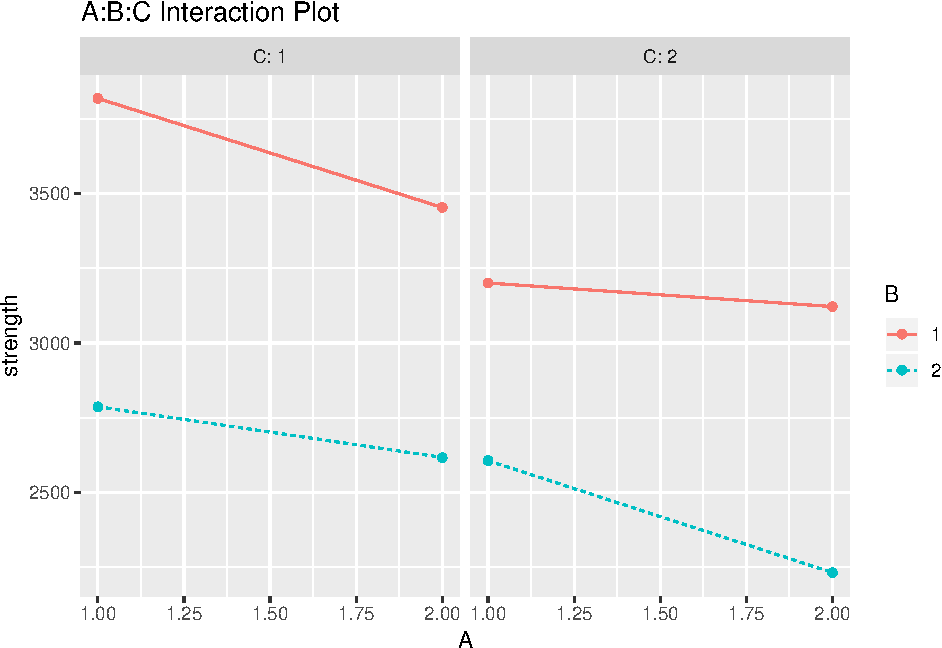
\includegraphics{Markdown_HW_7_files/figure-latex/unnamed-chunk-2-1.pdf}

\begin{Shaded}
\begin{Highlighting}[]
\KeywordTok{interaction.ABC.plot}\NormalTok{(strength, A, C, B, }\DataTypeTok{data =}\NormalTok{ paper.towel.strength)}
\end{Highlighting}
\end{Shaded}

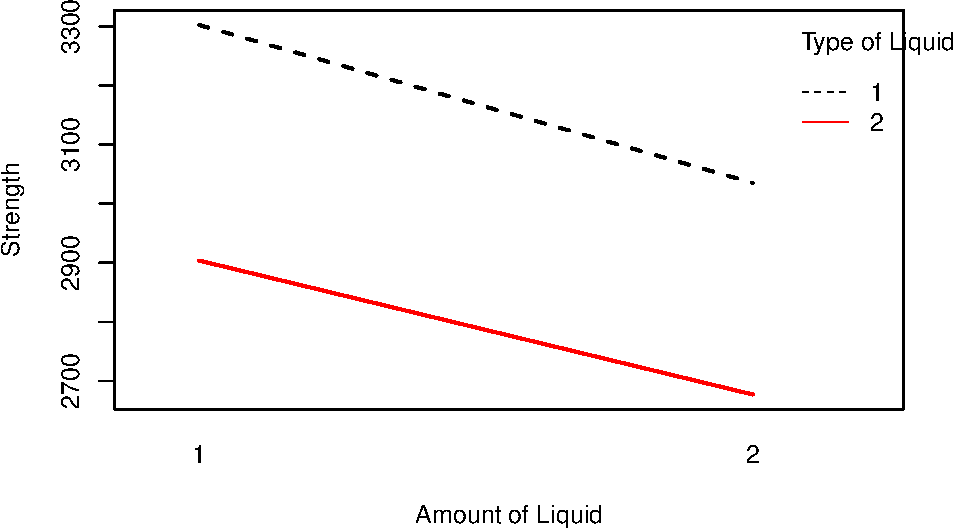
\includegraphics{Markdown_HW_7_files/figure-latex/unnamed-chunk-2-2.pdf}

\begin{Shaded}
\begin{Highlighting}[]
\KeywordTok{interaction.ABC.plot}\NormalTok{(strength, C, A, B, }\DataTypeTok{data =}\NormalTok{ paper.towel.strength)}
\end{Highlighting}
\end{Shaded}

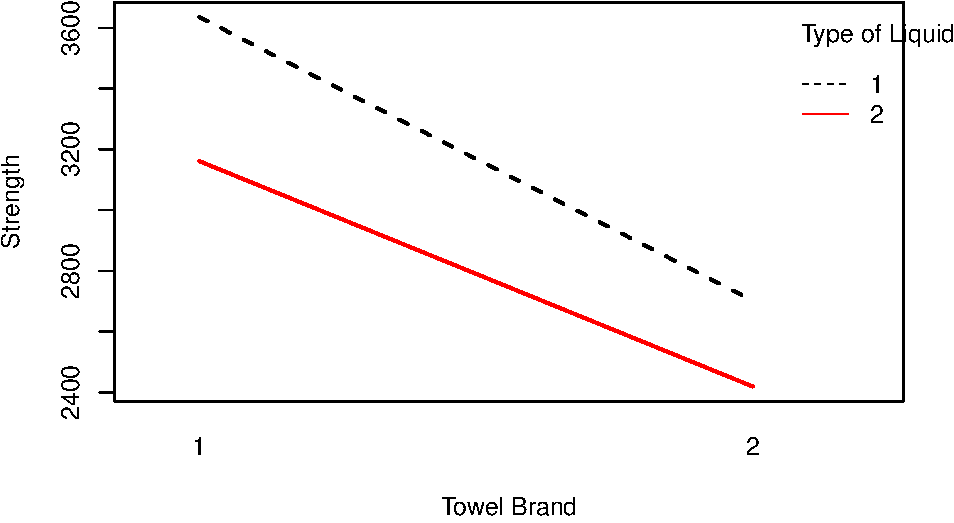
\includegraphics{Markdown_HW_7_files/figure-latex/unnamed-chunk-2-3.pdf}

\begin{enumerate}
\def\labelenumi{(\alph{enumi})}
\setcounter{enumi}{3}
\tightlist
\item
  Provide an analysis of variance table for this experiment, test the
  various effects, show plots of significant main effects and
  interactions, and draw conclusions.
\end{enumerate}

For part (d), proceed with the typical ANOVA, without variable
transformation, etc., regardless of your opinion on the residual plots
in (c). Test each effect in the ANOVA table at 0.01 (so you maintain a
FWER of 0.04). You do not need to produce plots of significant effects.

\begin{enumerate}
\def\labelenumi{(\alph{enumi})}
\setcounter{enumi}{4}
\tightlist
\item
  Construct confidence intervals for each of the treatment contrasts
  that you listed in part (b), using an appropriate method of multiple
  comparisons. Discuss the results. For part (e), use a confidence level
  of 99\% for the one primary contrast of interest
\end{enumerate}


\end{document}
